% Created:  Sun 15 Jun 2014 04:15 pm
% Modified: Wed 09 Jul 2014 03:02 PM
% @author Josh Wainwright
% File name : mainfile.tex

\documentclass[a4paper,9pt,twoside,twocolumn]{extarticle}
\usepackage[utf8]{inputenc}

%%% PAGE DIMENSIONS ------------------------------------------------------------
\usepackage[top=3cm,
	bottom=2cm,
	left=1.5cm,
	right=1.5cm]{geometry}
\usepackage[parfill]{parskip}
\setlength{\columnsep}{1.5em}

%%% HEADERS & FOOTERS ----------------------------------------------------------
\usepackage{fancyhdr}
\pagestyle{fancy}
\pagestyle{fancy}
\fancyhf{}
\fancyhead[LE,RO]{\thepage}
\fancyhead[RE,LO]{\leftmark}
\fancyfoot[CE,CO]{}
\fancyfoot[LE,RO]{}

%%% SECTION TITLE APPEARANCE ---------------------------------------------------
% \usepackage{sectsty}
% \allsectionsfont{\sffamily\mdseries\upshape}
\makeatletter
\@addtoreset{section}{part}
\makeatother

%%% PACKAGES -------------------------------------------------------------------
\usepackage[hypcap=false,
	font=small,
	labelfont=bf,
	textfont=it]{caption}
\usepackage{subcaption}
\captionsetup{subrefformat=parens}

\usepackage[pdftex]{graphicx}
\usepackage{booktabs}
\usepackage{array}
\usepackage{longtable}
\usepackage{tabu}
\usepackage{multirow}
\usepackage{verbatim}
\usepackage{listings}
\usepackage{xcolor}
\usepackage[binary-units]{siunitx}
\usepackage{amsmath}
% \usepackage[%
% 	activate={true,nocompatibility},
% 	final,
% 	tracking=true,
% 	kerning=true,
% 	spacing=true,
% 	factor=1100,
% 	stretch=10,
% 	shrink=10]{microtype}
% \microtypecontext{spacing=nonfrench}

%% CODE STYLING ----------------------------------------------------------------
\definecolor{dkgreen}{HTML}{4e9a06}
\definecolor{gray}{HTML}{555753}
\definecolor{mauve}{HTML}{75507b}
\definecolor{dkblue}{HTML}{3465a4}

\lstset{frame=tb,
  language=Java,
  aboveskip=3mm,
  belowskip=3mm,
  showstringspaces=false,
  captionpos=b,
  columns=flexible,
  basicstyle={\small\ttfamily},
  numbers=none,
  numberstyle=\tiny\color{gray},
  keywordstyle=\color{dkblue},
  commentstyle=\color{dkgreen},
  stringstyle=\color{mauve},
  breaklines=true,
  breakatwhitespace=true
  tabsize=3
}

%% BIBIOGRAPHY -----------------------------------------------------------------
\usepackage{cite}

%%% ToC (table of contents) APPEARANCE -----------------------------------------
\renewcommand{\contentsname}{Table of Contents}
% \setcounter{tocdepth}{2}

%%% PDF LINKS AND STYLE --------------------------------------------------------
\usepackage[bookmarks=true]{hyperref}
\hypersetup{%
	colorlinks=true, % false: boxed links; true: colored links
	linkcolor=black, % color of internal links (change box color with linkbordercolor)
	citecolor=black, % color of links to bibliography
	filecolor=black, % color of file links
	urlcolor=black   % color of external links
}
\hypersetup{pdftitle={Josh Wainwright MSc Project},
	pdfauthor={Josh Wainwright}}

%*******************************************************************************
%******************************** END HEADER ***********************************
%*******************************************************************************

\begin{document}

\graphicspath{{front/} {intro/} {grid/} {quadtree/} {clusters/} {plugin/}
	{build/}}

% Created:  Sun 15 Jun 2014 04:29 pm
% @author Josh Wainwright
% File name : titlepage.tex

\newgeometry{margin=1in}
\begin{titlepage}
	\begin{center}
		\vspace*{\fill}

		\centering
		\includegraphics[scale=1.0]{Logo.pdf}
		\vfill

		\hrule
		{\LARGE\bf Medical Image Processing with Quadtrees\\[0.4cm]}
		\hrule

		\vfill
		\large
		School of Computer Science\\
		University of Birmingham

		\vfill
		Josh Wainwright
		\vfill

		\vfill
		\textit{Supervisor:} Iain Styles \\
		\vfill
		\textit{Date:} September 2014
		\vfill
		\vfill

	\end{center}
\end{titlepage}
\restoregeometry%

\newgeometry{onecolumn}
\thispagestyle{empty}

\textbf{Title:} Medical Image Processing with Quadtrees \\
\textbf{Author:} Josh Wainwright \\
\textbf{Supervisor:} Iain Styles \\
\textbf{Date:} September 2014 \\
\textbf{}
\vfill
Completed as part of a Post Graduate Masters Degree in Computer Science at the
University of Birmingham (2013/2014).

\pagenumbering{roman}

% \newgeometry{left=5cm, top=5cm, right=5cm}
\thispagestyle{empty}
\part*{Abstract}
\label{prt:abstract}
\addcontentsline{toc}{section}{Abstract}

This project introduces the concept of data clustering and it's uses in medical
and biological image analysis and examines some existing techniques for
extracting clustering information from such data sets. A new technique based on
quadtree style data structures is discussed and an implementation tested and
evaluated based on this technique. This method is found to perform well even
under difficult conditions, such as noisy data, where others struggle, though
has limitations in data set size, resource usage and taking advantage of
parallel processing.

% \restoregeometry

\clearpage

\thispagestyle{empty}
\tableofcontents
\addcontentsline{toc}{section}{Table of Contents}
\thispagestyle{empty}
\listoffigures
\addcontentsline{toc}{section}{List of Figures}
\thispagestyle{empty}
\listoftables
\addcontentsline{toc}{section}{List of Tables}
\thispagestyle{empty}
\lstlistoflistings%
\addcontentsline{toc}{section}{List of Code Listings}
\thispagestyle{empty}

\restoregeometry
\clearpage
\pagenumbering{arabic}
% \twocolumn


% Created:  Sun 15 Jun 2014 04:25 pm
% Author:   Josh Wainwright
% Filename: introduction.tex
\part{Introduction}
\label{prt:introduction}

\section{Medical Imaging}
\label{sec:section_name}

% TODO reword first sentence.
In various scientific fields, viewing and imaging objects smaller than the
human eye can naturally observe, is an ability eagerly sought. Microscopy in
medical fields has allowed us to learn about the nature of tissues,
micro-organisms and cells and the way they work together and to develop
preventative measures and cures for injuries and diseases.

The humble microscope, used as far back as the 1500's, is able to show us a
world that is not usually visible. In recent times, as our understanding has
grown, we have desired to see beyond what ordinary microscopes are capable of
and have invented machines that let us catch a glimpse of some of the smallest
structures in biology---molecules. However, when the objects to be viewed get
this small, of the order of a few tens of nanometers, the light that is used to
view them becomes the limiting factor.

% \section[Sub-Diffraction-Limit Imaging]{Sub-Diffraction-Limit\\ Imaging}
\section{Sub-Diffraction-Limit Imaging}
\label{sec:sub_diffraction_limit_imaging}

Imaging objects becomes more difficult as they get smaller because of the
wavelength of light ($\lambda$). Once two objects are separated by a distance
of an order similar to that of the wavelength of the light used to view them,
it is no longer possible to resolve these two objects apart. Instead all that
can be seen is a blur of the two objects together.

There have been several techniques developed for distinguishing objects apart
on smaller and smaller scales. Many of these involve using different
wavelengths of light.  For example, instead of being limited by visible light,
$\lambda \approx 5\times 10^{-7} \textrm{m}$, x-ray radiation ($\lambda \approx
10^{-10} \textrm{m}$) or even electrons ($\lambda \approx 10^{-11} \textrm{m}$)
can be used to resolve smaller scales in x-ray and electron microscopy
respectively. The smaller wavelengths imply higher energies however, meaning
that there is the danger of destroying the sample.

The minimum separation at which two objects can be resolved is given by Abbe's
criterion, $d$,

\begin{align}
	d &= \frac{\lambda}{2N\!A} \\
	  &= \frac{\lambda}{2n\sin\theta},
\end{align}

where $N\!A$ is the numerical aperture of the microscope, the range of angles
that the microscope's lens will let light through properly, $n$ is the
refractive index of the lens material and $\theta$ is the angle at which the
light is incident on the lens. For typical values of $\lambda \approx
\SI{500}{\nano\metre}$ (in the middle of the visible range), and $N\!A = 1.5$,
the maximum resolving distance is $d = \SI{160}{\nano\meter}$, this is the
diffraction limit. This is an order of magnitude larger than the objects that
need to be resolved. A few attempts to avoid this limit using exotic types of
lenses have been developed\cite{fang2005sub}, but these are currently far more
expensive to use than traditional imaging equipment.

\subsection{Image Manipulation}
\label{sub:image_manipulation}

Instead of trying to avoid the diffraction limit using shorter wavelengths of
light or particles, other techniques employ different methods of actually
capturing the image, and/or cleaver manipulation of the images that are
produced to get around the limitations of the diffraction problem.

For example Stochastic Optical Reconstruction Microscopy (STORM)
\cite{rust2006sub} and Photo-Activation Localisation Microscopy
(PALM)\cite{owen2010palm} use a technique where the objects to be imaged are
molecules of a fluorescent dye. These are attached to the object of interest, a
cell or sample of tissue for example. The type of dye molecule used allows the
fluorescence to be switched on and off, allowing some markers to be imaged
separately to others, effectively increasing the distance between points. Once
an image is captured, the point spread function (PSF) of the image of a marker
is used to locate the single point location of that marker, the ``on'' markers
are turned off and different ones turned on and the image retaken.  When many
of these images are taken, they can be combined to provide accurate information
on the original location of the markers and hence the shape and dimensions of
the object.

\begin{figure}[tbh]
	\centering
	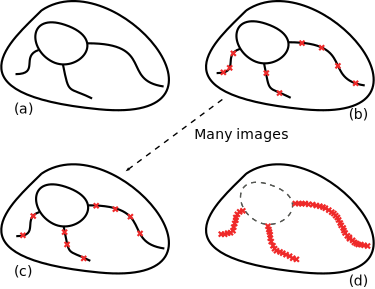
\includegraphics[width=7cm]{STORM.pdf}

	\caption[Creation of a STORM image.]{STORM imaging. (a) The actual
		structure to be imaged is too small for regular microscopy. In stages
		(b) through (c), many images are taken, each with a different subset of
		the fluorescent markers activated. When the images are combined, (d),
		the points add up and reveal the nature of the object.}\label{fig:STORM}
\end{figure}

The aim of this project is to provide a means by which the results of this
method of imaging can be analysed more efficiently and with a greater degree of
accuracy. This will take the form of a plugin for a piece of popular image
processing software called ImageJ.

The main deliverable is a plugin for extracting clusters of points from large
data sets for ImageJ. This plugin is written in Java and makes use of the
ImageJ Java API\cite{imagejapi}.

The sections included in this report are detailed below.

\begin{description}
	\item[\fullref{prt:introduction}] \hfill \\
		A brief background to the project with information about the type of
		data to be managed.

	\item[\fullref{prt:existing_cluster_analysis_algorithms}] \hfill \\
		A discussion of the existing algorithms that are in use for different
		applications and the reasons they do not fulfill the requirements of
		this project.

	\item[\fullref{prt:custom_algorithm}] \hfill \\
		A detailed examination of the algorithms that are developed in this
		project and the ways in which they are superior to the existing
		algorithms available.

	\item[\fullref{prt:imagej_plugin}] \hfill \\
		An explanation of the plugin that was developed for this project with
		information about how the constraints and variables of the algorithms
		are implemented in the plugin.

	\item[\fullref{prt:evaluation}] \hfill \\
		An evaluation of the success of the product at fulfilling the
		requirements given as well as of the processes and schedules that were
		followed during the project.

	\item[\fullref{prt:appendix}] \hfill \\
		A number of additional pieces of information and derivations to
		supplement the information in the body of this report.
\end{description}

% Created:  Sun 22 Jun 2014 11:25 AM
% @author Josh Wainwright
% File name : benchmarking.tex

\section{Benchmarking}
\label{sec:benchmarking}

Throughout the project, a set of files will be used to test the algorithms
that are developed; their correctness and effectiveness, speed and resource
use.  These files contain real data formated in the same way as would be
expected for data given to the plugin in general use. The files that will be
used are detailed in Table~\ref{tab:benchmarking-files}.

\renewcommand{\arraystretch}{1.3}
\begin{table}[htbp]
\centering
\begin{tabular} {l c r}
	\toprule
	File Name & Size & Points \\
	\midrule
	\texttt{palm-1.txt} & \SI{12}{\mebi\byte} & 65572 \\
	\texttt{palm-2.txt} & \SI{6.4}{\mebi\byte} & 36672 \\
	\texttt{palm-3.txt} & \SI{5.8}{\mebi\byte} & 33342 \\
	\texttt{palm-3-small.txt} & \SI{176}{\kibi\byte} & 1000 \\
	\texttt{uniform.txt} & \SI{22}{\mebi\byte} & 2000000 \\
	\bottomrule
\end{tabular}

\caption{These files containing sample data are used for benchmarking
	throughout the project.}\label{tab:benchmarking-files}
\end{table}

Note that \texttt{palm-3-small.txt} is a subset of \texttt{palm-3.txt} which
is used for simply checking correctness of algorithms. A summary of the
columns that are included in the files, used and unused fields, is included in
Appendix~\ref{app:data_file_structure}.

% TODO system information of benchmark machine
%
\begin{tabular}{l l}
	Architecture:          & x86\_64 \\
	CPU op-mode  (s):      & 32-bit, 64-bit \\
	Byte Order:            & Little Endian \\
	CPU (s):               & 4 \\
	On-line CPU (s) list:  & 0--3 \\
	Thread (s) per core:   & 1 \\
	Core (s) per socket:   & 4 \\
	Socket (s):            & 1 \\
	NUMA node (s):         & 1 \\
	Vendor ID\@:           & GenuineIntel \\
	CPU family:            & 6 \\
	Model:                 & 60 \\
	Stepping:              & 3 \\
	CPU MHz:               & 800.000 \\
	BogoMIPS\@:            & 6385.81 \\
	Virtualization:        & VT-x \\
	L1d cache:             & 32K \\
	L1i cache:             & 32K \\
	L2 cache:              & 256K \\
	L3 cache:              & 6144K \\
	NUMA node0 CPU (s):    & 0--3 \\
\end{tabular}

% Created:  Tue 01 Jul 2014 03:19 PM
% Modified: Tue 01 Jul 2014 03:19 PM

\part{Data Structures}
\label{prt:data_structures}

%TODO
The way in which the data is represented in memory


% Created:  Mon 23 Jun 2014 13:15 PM
% Modified: Fri 27 Jun 2014 12:11 PM

\section{Simple Grid Method}
\label{sec:simple_grid_method}

The simplest method for analysing the distribution of points is to use a
regular grid of cells and place the points into the cells one at a time. Once
all points have been added, the number of points per cell can be treated as a
greyscale birghtness value. This gives a simple pixel-image, with brightness as
a function of density, in the pnm image format. A thresholding filter can then
be applied to remove the points that are isolated and leave the denser areas
coresponding to clusters.

Though the resolution of this method can be easily changed by altering the size
of the cells and the grid, it performs badly when presented with data that is
even slightly noisy. If the clusters themselves have a density that is not
significantly above the background noise level, the thresholding step is prone
to either exclude much of the real data, or to increase the size of the
clusters by including too much noise. These two effects can be seen clearly in
Figure~\ref{fig:grid-noise}, where \texttt{palm-1.txt} was used with a cell
size of 200. The range of the data is from 0 to 41000 for both the $x$ and the
$y$ axes, thus the images are 205 by 205 pixels. This data took
\SI{0.495}{\second} to generate.

\begin{figure}[ht]
    \centering
    \begin{subfigure}[b]{0.48\linewidth}
        \frame{\includegraphics[width=\textwidth]{grid-noise-low.png}}
        \caption{}\label{fig:grid-noise-low.png}
    \end{subfigure}%
    \quad
    \begin{subfigure}[b]{0.48\linewidth}
        \frame{\includegraphics[width=\textwidth]{grid-noise-high.png}}
        \caption{}\label{fig:grid-noise-high.png}
    \end{subfigure}
    \caption{Setting a low threshold, \subref{fig:grid-noise-low.png}, means
    that many of the points in the clusters are lost. Setting it higher,
    \subref{fig:grid-noise-high.png}, includes too many of the points deemed to
    be noise.}\label{fig:grid-noise}
\end{figure}

% Created:  Fri 27 Jun 2014 11:24 AM
% Author:   Josh Wainwright
% Filename: quadtree.tex

\section{Quadtrees}
\label{sec:quadtrees}

Since the simple grid method described in Section~\ref{sec:simple_grid_method}
performs slowly and does not offer good cluster analysis, a different approach
is needed. The chosen method is to use a quadtree data structure.

Quadtrees are a type of recursive abstract data type in the form of a tree
where every node has exactly zero or four children. A node with zero children
is a leaf and contains some information, value or quantity. A node with four
children is not a leaf and cannot hold information.

Quadtrees are often used in image processing since the four children of the
root node can naturally represent the four quadrants of an image; upper left,
upper right, lower left and lower right. Since each of these children is also a
quadtree, the image can be subdivided to any arbitrary depth. From this point,
information about the image can be ``seen'' more easily by the computer and
statistics calculated.

\subsection{Quadtree Definitions}
\label{sub:quadtree_definitions}

It is useful to define a few terms that shall be used in the context of
quadtrees. Many of these are identical to the definitions more commonly applied
to binary trees.

\begin{description}
	\item[Node] (Cell, element) A leaf in the tree which holds some
		information, value or quantity.
	\item[Root Node] The node at the topmost position in the tree. It has no
		parents and is never a leaf.
	\item[Child] One of the four nodes that are beneath a given node for which
		there is a direct path of length 1 between this node and it.
	\item[Height] The length of the longest path from the root node to one of
		the leaf nodes.
	\item[Depth] The length of the path from a given node up to the root.
	\item[Completeness] A quadtree is `complete' when each of the root node's
		four children have the same height. In this case, the number of leaves
		in the tree is a maximum.
	\item[Quadtree Code] (Code) A unique number or value that is assigned to a
		node by adding its position with respect to its siblings to the code of
		its parent.
\end{description}

\subsection{Code Orderings}
\label{sub:code_orderings}

In order to identify a node uniquely in the tree, each node is given a code
that is built up from it's parent's code plus some value that identifies it
among it's siblings. The root node is usually chosen to have an empty code so
that the first four children are given the first level codes.

The choice of what order to label the children is important if the order
in which the nodes are placed is important. For spatial indexing, for example,
each node represents a quadrant in two dimensional space, so being able to
traverse the children in a sensible and predictable way is essential.

\begin{figure}[tbhp]
	\centering
	\begin{subfigure}[b]{3.5cm}
		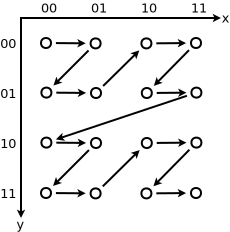
\includegraphics[width=\textwidth]{traverse-z-order.pdf}
		\caption{}\label{fig:traverse-z-order.pdf}
	\end{subfigure}%
	\quad
	\begin{subfigure}[b]{3.5cm}
		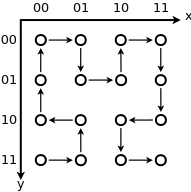
\includegraphics[width=\textwidth]{traverse-hilbert-order.pdf}
		\caption{}\label{fig:traverse-hilbert-order.pdf}
	\end{subfigure}
	\\[0.2cm]
	\begin{subfigure}[b]{3.5cm}
		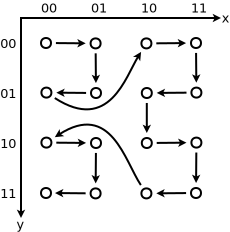
\includegraphics[width=\textwidth]{traverse-gray-order.pdf}
		\caption{}\label{fig:traverse-gray-order.pdf}
	\end{subfigure}%
	\quad
	\begin{subfigure}[b]{3.5cm}
		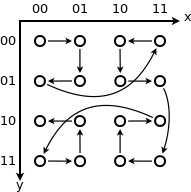
\includegraphics[width=\textwidth]{traverse-modgray-order.pdf}
		\caption{}\label{fig:traverse-modgray-order.pdf}
	\end{subfigure}

	\caption[A selection of possible tree traversal orderings]{A selection of
		possible tree traversal orderings. Each of theses is, more formally, a
		space filling curve which is a direct, unique mapping from a 2D grid to
		a 1D array. \subref{fig:traverse-z-order.pdf} shows Z-order,
		\subref{fig:traverse-hilbert-order.pdf} shows Hilbert order,
		\subref{fig:traverse-gray-order.pdf} shows Gray code order and
		\subref{fig:traverse-modgray-order.pdf} shows the modified Gray code
		order developed for this project.}\label{fig:order_traversals}
\end{figure}

\subsubsection[Morton Order]{Morton Order (Z-Order)}
\label{ssub:morton_code_z_order_}

Perhaps the most natural order to give to the values in a spatial quadtree is
to number them from 1 to 4, left to right, top to bottom. This can be made more
appropriate for a computer to use by changing to zero based indexing,
numbering from 0 to 3. This is called Morton Order\cite{mortoncomputer} or
Z-order because of the resulting path that would be followed by traversing the
nodes in order, Figure~\ref{fig:traverse-z-order.pdf}. This has several useful
features.

\begin{enumerate}
	\item First, the numbers can be converted to base 2; 0 becomes 00, 1
		becomes 01, 2 becomes 10, and 3 becomes 11.

	\item This has advantages since binary is very efficient for computers to
	work with and allows certain tricks to be employed (see Morton Order
	Coordinates below).

	\item Also, this numbering system is easily extendible to any depth of
	tree that can be imagined.

	\begin{enumerate}
		\item The root, as mentioned before, is given no value,
		\item each of the children are numbered {00} through 11.

		\item the children of these children are numbered 00 to 11 with the
		parent as a prefix. So the children of node 00 are 0000, 0001, 0010
		and 0011. Likewise, the children of 11 are 1100, 1101, 1110 and 1111.

		\item The children are always numbered in the same order. If starting
		at the top and going top to bottom and left to right, this is
		maintained for all children.
	\end{enumerate}
\end{enumerate}

\subsubsection*{Morton Order Coordinates}
\label{ssub:morton_order_coordinates}

Another useful feature of the Morton ordering is the simple conversion from
quadtree code to Cartesian coordinate notation. The steps to convert to
coordinate form are:

\begin{enumerate}
	\item Ensure the code is in binary format with two bits for each level of
		the tree.
	\item \emph{De-interleave} the bits of the code (starting with the first
		being given to the $y$-axis, assign bits to the $y$ and $x$ axes
		building up a binary value for each).
	\item Convert the resulting two binary value to decimal to give a standard
		decimal $(x,y)$ Cartesian coordinate.
\end{enumerate}

These steps result in a coordinates that represents the top left corner of the
node. The coordinate is dependant on the length of the code, so to compare two
coordinated from their codes, the codes must be of the same length.

\begin{figure}[tbhp]
	\centering
	\includegraphics[width=3cm]{deinterleave.pdf}

	\caption[Decomposition of a Z-order code to give coordinates.]{Decomposition
		of a Z-order code using de-interleaving to give Cartesian coordinates.
		The bits of the code are alternately assigned to the y- and then
		x-coordinate which is then converted to decimal to given the final
		coordinate of the cell.}\label{fig:deinterleave}
\end{figure}

This method means that it is very easy to calculate an arbitrary number of
nodes in any direction by simply converting the code for a node to coordinates,
adding or subtracting the number of positions to move in the $x$ and $y$
directions and then converting back to quadtree code representation by
following the algorithm above in the reverse order.

Of course, this method has no knowledge of the structure of the quadtree being
used and so only provides the code of the node that would occupy the space at
the given coordinate. That node might not exist---the tree might not extend
deep enough, so the node in that position is larger than expected; or the tree
might be deeper at that location meaning the node is smaller. In these cases,
there are a number of options as to how to find the correct node for the code:

\begin{itemize}
	\item The code can be shortened and/or lengthened and the resulting adapted
		code checked to see if it is in the tree. This trial and error method
		can be fastest when there is a limit on the depth range allowed when
		searching (see Section~\ref{sub:algorithm_description}).
	\item The tree can be traversed, starting at the root, to find the nearest
		node to the expected code reference.
\end{itemize}

The first of these is used in the plugin since it allows the hash map structure
to be used when searching which speeds up the process.

\subsubsection{Hilbert Order}
\label{ssub:hilbert_order}

One of the reasons the Z-order above becomes difficult to work with is that
the resulting path from traversing the nodes in-order has to make large jumps
and so cells which are numbered next to each other may, in fact, not be near
each other in the image. This property is known as being continuous.

A number of routes exist that avoid this jumping around the image. These are
based on space filling curves which have the property of being simple recursive
patterns that visit every point in a 2D space exactly once. These curves were
first discovered in the early 1900's and described mathematically by David
Hilbert\cite{hilbert1970stetige}. One of the curves that Hilbert found, the
Hilbert Curve, is particularly useful since it can be represented in the
simplest level in a two by two square which is then recursively repeated for
each quadrant of that first square---exactly as the quadtree is.

The path that the traversal of points follows becomes fairly complicated,
Figure~\ref{fig:traverse-hilbert-order.pdf}, meaning that the calculation of
neighbours becomes difficult as there is no simple way to traverse the path an
arbitrary distance. Two of the neighbours are always simple to find by simply
going a single step forward and backward, but the others are far more complex.

\subsubsection{Gray Codes}
\label{ssub:gray_codes}

The Gray Code, developed by Frank Gray in 1953\cite{gray1953pulse}, was
originally designed to reduce the error rate produced by mechanical
electronics. The code is a variation on binary where each step, when
incrementing, changes only a single bit at a time. This meant that
electromechanical apparatus was less likely to make a mistake or generate
errors since the actions required to count from one to two required only a
single bit change, rather than two, which would be required for binary
counting.  When using just two bits, i.e., counting from zero to three, the
steps are very similar to binary, (00, 01, 11, 10).

The path that this follows is shown in
Figure~\ref{fig:traverse-gray-order.pdf}. This does not seem to provide any
benefits since there is now more jumping around the image space than with
Z-order and the neighbours are just as difficult to calculate as for Hilbert
Order. However, by using a different arrangement for each of the sub-trees, as
the Hilbert curve does, the leaf nodes group themselves in a very ordered
fashion.  When arranged as in Figures~\ref{fig:traverse-modgray-order.pdf}
and~\ref{fig:modgray-traversal}, each cell is arranged such that the codes for
any two neighbouring nodes at the same depth differs by exactly one bit. This
means that checking if any two nodes are neighbours becomes trivial.

\begin{figure}[tbhp]
	\centering
	\begin{subfigure}[c]{3.4cm}
		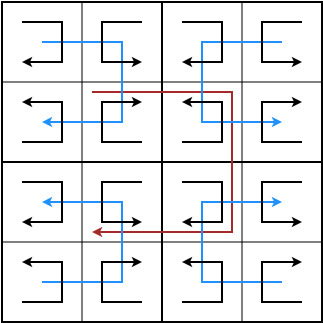
\includegraphics[width=\textwidth]{modgray-2-levels-arrows.pdf}
		\caption{}\label{fig:modgray-2-levels-arrows.pdf}
	\end{subfigure}%
	\quad
	\begin{subfigure}[c]{4.6cm}
		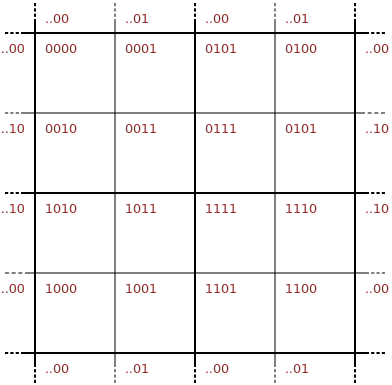
\includegraphics[width=\textwidth]{modgray-2-levels-numbers.pdf}
		\caption{}\label{fig:modgray-2-levels-numbers.pdf}
	\end{subfigure}

	\caption[Modified Gray Code ordering]{The tree traversal that was developed
		for this project is a variation of the Gray code order discussed in
		Section~\ref{ssub:gray_codes}.  Instead of all sub-quadrants having the
		same orientation, each is reflected in either the x- or y-axis,
		\subref{fig:modgray-2-levels-arrows.pdf}. This has the advantage that
		neighbouring nodes have codes which differ by exactly one bit,
		\subref{fig:modgray-2-levels-numbers.pdf}.}\label{fig:modgray-traversal}
\end{figure}

% \begin{figure}[tbhp]
% 	\centering
% 	\includegraphics[width=7.4cm]{modgray-steps.pdf}
% 	% TOD short caption
% 	% TOD caption
% 	\caption{modgray-Steps}\label{fig:modgray-steps}
% \end{figure}

\subsubsection{Other Orderings}
\label{ssub:other_orderings}

As well as the orderings discussed above, there are also a number of other
space filling curves and dis-joint orderings that were discounted.
Figure~\ref{fig:modgray-2-alternatives} shows some of these.

\begin{itemize}

	\item Figure~\ref{fig:modgray-alt-order.pdf} shows \emph{row order}
		traversal of the grid. This is extremely simple to implement for a
		simple grid-like arrangement, but is very awkward and looses much of
		the information when using quadtrees.

	\item Figure~\ref{fig:modgray-alt-prime.pdf} shows \emph{row-prime order},
		also known as snake-order\cite{goodchild1983optimizing}, traversal.
		This is a slight modification of row order which is continuous but,
		again, is not recursive so not suitable for use with quadtrees.

	\item Figure~\ref{fig:modgray-alt-rotated.pdf} is identical to them
		modified Gray order above, but with a single \SI{90}{\degree} rotation.
		Since the orientation of an image has no effect on the clusters found,
		all rotations and reflections provide the same functionality as the
		original. The particular form chosen is simply due to {\ae}sthetic
		preference.

	\item Figure~\ref{fig:modgray-alt-pinwheel.pdf} shows an alteration to the
		modified Gray code order, named \emph{pinwheel order}, where, instead of
		reflecting the quadrants, each is rotated about it's center
		\SI{90}{\degree} so that the whole image is rotationally symmetric,
		something the modified Gray code lacks.  This form turns out not to
		provide any additional features and makes conversion from quadtree code
		to coordinate representation substantially more difficult.

\end{itemize}

\begin{figure}[tbhp]
	\centering
	\begin{subfigure}[b]{3.5cm}
		\includegraphics[width=\textwidth]{modgray-alt-order.pdf}
		\caption{}\label{fig:modgray-alt-order.pdf}
	\end{subfigure}%
	\quad
	\begin{subfigure}[b]{3.5cm}
		\includegraphics[width=\textwidth]{modgray-alt-prime.pdf}
		\caption{}\label{fig:modgray-alt-prime.pdf}
	\end{subfigure}
	\\[0.2cm]
	\begin{subfigure}[b]{3.5cm}
		\includegraphics[width=\textwidth]{modgray-alt-rotated.pdf}
		\caption{}\label{fig:modgray-alt-rotated.pdf}
	\end{subfigure}%
	\quad
	\begin{subfigure}[b]{3.5cm}
		\includegraphics[width=\textwidth]{modgray-alt-pinwheel.pdf}
		\caption{}\label{fig:modgray-alt-pinwheel.pdf}
	\end{subfigure}

	\caption[Alternative quadtree orderings.]{There are a number of different
		space filling curves that can be used to map a two dimensional grid to
		a single dimensional array. To be considered for use in the quadtree
		ordering, the new ordering must provide some improvement of efficiency
		of some operations. Here are shown some orderings which were
		discounted.}\label{fig:modgray-2-alternatives}
\end{figure}

\subsubsection{Chosen Ordering}
\label{ssub:Chosen Ordering}

Despite the promising features of the modified Gray ordering, the simple Morton
ordering is used when constructing quadtrees in the ImageJ plugin. This is due
to the issues encountered when developing a method of discovering neighbours of
nodes in the modified Gray code system. It was found that, despite there being
an assurance that two neighbours' codes differ by exactly one bit, this cannot
provide a one to one mapping with the required neighbours of that node.

Consider, for example, a node, $S$, at a depth of three in the tree where the
rook's case neighbours (see Section~\ref{sub:choosing_neighbours}) are
required. This node has a code consisting of 6 bits, two for each level. From
this code, a total of six possible neighbour candidates can be identified by
simply flipping each of the bits in the code.  These neighbours are shown for
an example node in Table~\ref{tab:s-neighbours} and their position relative to
the original shown in Figure~\ref{fig:modgray-failures}. The first two of these
possible neighbours, the results of flipping the two least significant bits,
are guaranteed always to be valid neighbours since they share the same parent
as $S$. However, the two other neighbours which need to be selected from the
remaining four possibilities, cannot be identified easily.  These other
possible neighbours exist at other locations in the quadtree, always either
vertically above or below or horizontally to the left or right of $S$, but
there is no simple test to determine if they are actually neighbours or not.

\begin{table}
	\centering
	\begin{tabu}{c c c}
		\toprule Node $S$ & Neighbours \\
		\cmidrule{1-2} \multirow{6}{*}{101001}
		& 10100\textbf{0} & \rdelim\}{2}{4cm}[Guaranteed to be neighbours] \\
		& 1010\textbf{1}1 & \\
		& 101\textbf{1}01 & \rdelim\}{4}{4cm}[Must choose two others]\\
		& 10\textbf{0}001 & \\
		& 1\textbf{1}1001 & \\
		& \textbf{0}01001 & \\
		\bottomrule
	\end{tabu}
	\caption[The possible neighbours for a node using modified Gray
		ordering.]{The possible neighbours for a node using modified Gray
		ordering. The bit that was flipped is highlighted for each
		neighbour.}\label{tab:s-neighbours}
\end{table}

\begin{figure}[tbhp]
	\centering
	\includegraphics[width=8.8cm]{modgray-failures.pdf}
	\caption[Flipping code bits gives too many possible neighbours.]{Flipping
		the bits of the code to get possible neighbours gives too many
		possibilities to be able to select the correct neighbours. This problem
		is exaggerated as the node gets deeper in the tree since there are more
		bits in the code to change. The incorrect neighbours are always in line
		with the original and represent what would be neighbours if the tree
		was some number of levels shallower.}\label{fig:modgray-failures}
\end{figure}

\subsection{Constructing Orderings in Code}
\label{sub:constructing_orderings_in_code}

Since the quadtree is a recursive data structure, it is necessary to be able to
maintain the correct orientation of child trees with respect to their parents
at the construction stage. It turns out that this is easy to achieve and thus
adapting it for each of the arrangements discussed above is simply a matter of
adjusting the next part of the code that is added for each of the four children
when creating them. Pseudo code to achieve this for Morton order is shown in
Listing~\ref{code:child-construction}. The constructor for a quadtree is
\texttt{Quadtree(max\_x, max\_y, code)}, where \texttt{code} is the new portion
of code to be added for that child.

\begin{center}
\begin{minipage}{\textwidth}
\begin{lstlisting}[caption={[Code to generate the children of the current
	quadtree using Z- and Gray ordering.]Code to generate children of the
	current quadtree while maintaining the correct ordering. Z- and Gray
	ordering.}, label=code:child-construction]
	// Child creation,  Z-Order
	t_l = new Quadtree(100, 100, this.code + "00");
	t_r = new Quadtree(100, 100, this.code + "01");
	b_l = new Quadtree(100, 100, this.code + "11");
	b_r = new Quadtree(100, 100, this.code + "10");

	// Child creation,  Gray Code
	t_l = new Quadtree(100, 100, this.code + "00");
	t_r = new Quadtree(100, 100, this.code + "01");
	b_l = new Quadtree(100, 100, this.code + "10");
	b_r = new Quadtree(100, 100, this.code + "11");
\end{lstlisting}
\end{minipage}
\end{center}

\subsection{Hash Table Implementation}
\label{sub:hash_table_implementation}

In order to speed up the subsequent operations applied to the quadtree
structure, it can be converted to a simpler, one dimensional data structure.
The method discussed above, to number the cells in a logical fashion based on
the code of the parent, can be viewed as a way to map the two dimensional image
to a single unique binary code, and hence to a one dimensional format. Thus,
the quadtree can be easily converted to an array structure by simply using the
key code as the array index. Once this is performed the access complexity is
significantly reduced. This operation is only performed once after the quadtree
has been generated meaning the amortized complexity is reduced.

As mentioned on page~\pageref{prt:custom_algorithm}, using a na\"{\i}ve
implementation has the potential to have a very poor space usage if the image
is not densely populated (in which case it is likely that few clusters would be
identifiable anyway). Instead, an implementation is created that makes use of
the \emph{hash table} data structure\cite{cormen2001introduction}. This allows
the data structure to increase in size dynamically as more space is needed, but
also provides linear time complexity for access, modification and search. The
quadtree code is used as the key for the hash table, and the data stored within
the cell with that code is the hash table value.

Using this data structure means that several operations are significantly sped
up. For example, for the quadtree format, the steps required to check if a
given code is present involves traversing the tree as specified by the code to see if a node with that code is found, thus a time
complexity of $O(\log n)$.  However, for a hash table, the hash function is
used to get a hash of the code to be checked and the appropriate location
checked. If the codes match, then the code does appear in the tree, a total of
two operations, and so constant $O(1)$.

Since the quadtree structure is defined recursively, it is not possible to
directly access a given location of the data. Instead it must be arrived at by
starting at the root, and, for every level, deciding which of the children the
destination exists in. This would be a time consuming step for a number of
operations, but the biggest effect would be when checking the neighbours of
cells since for every neighbour of every node, the tree must be traversed. This
is not an issue for the hash table since the single dimensional nature means
that data anywhere can be accessed directly.

Little spatial information should be lost during the conversion from quadtree
to hash table since this is all contained in the quadtree code assigned to the
node during the quadtree generation step. However, the quadtree representation
can be kept in memory for some processes. For example, to get all of the leaf
nodes of a given node, it is enough to start at that node and traverse the tree
in post- or pre-order and return the nodes that are arrived at, $O(\log n)$,
whereas, for the hash table, each node must be checked to decide if it is a
child, $O(n)$.

A hash table requires two pieces of information for each entry: a \emph{key}
and a \emph{value}. The key is what is used to locate items, its hash is used
as the index of the internal array. The value is the information that should be
accessible when using the key. For this application, since more than a single
piece of information should be accessible for each quadtree code, an object is
stored against each key. This has the format shown in
Table~\ref{tab:hashmap-columns}.

\begin{table}[htbp]
	\centering
	\begin{tabu}{l >{$\bullet$\hspace*{\tabcolsep}}p{0pt} p{5.4cm}}
		\toprule
		Key  & \multicolumn{2}{l}{Value} \\
		\midrule
		Quadtree Code && Set of points in this node \\
		              &&  Cluster ID that these points exist in \\
		              &&  Dimensions of this node \\
		              &&  Number of edges this node contributes to the
		                  perimeter of the cluster\\
		\bottomrule
	\end{tabu}

	\caption[Hash map key and value format for a quadtree.]{A hash map is used
		to associate a quadtree code with the required data for each node. The
		hash map value is an object containing several fields.}\label{tab:hashmap-columns}
\end{table}

% Created:  Wed 09 Jul 2014 03:00 PM
% Modified: Wed 09 Jul 2014 03:00 PM
% @author Josh Wainwright
% File name : clusters.tex

\part{Cluster Analysis}
\label{prt:cluster_analysis}

Cluster analysis is the grouping of a set of objects or items in a spatially or
informationally logical way such that the items that are placed in the same
group are more similar to each other than they are to the objects in the other
groups in the set. These groups shall be called \emph{clusters}. When dealing
with images, the clustering that is of interest is based on spatial location,
i.e., clusters should be composed of objects that are close together in the
image and clusters should be separated by regions of emptiness or background
level noise.

One of the primary reasons for chosing the quadtree method over the simple grid
methods was that the simple act of placing the objects, in this case
coordinates of data points, into the quadtree starts the process of analysing
the data. Since the points end up in a tree structure with the number of points
closely separated being on the lowest levels of the tree, the data is already
clustered in a way.

There are a number of alternative methods of identifying clusters in images.

% Created:  Mon 30 Jun 2014 05:32 PM
% Modified: Thu 31 Jul 2014 10:16 AM
% @author Josh Wainwright
% File name : rolling-ball.tex

\section{Rolling Ball Analysis}
\label{sec:rolling_ball_analysis}

The accessible surface area (ASA) algorithm, also known as the ``Rolling Ball
Method'', is a technique used in image processing for describing the outer
limit of a cluster of points. It is derived from biological molecules analysis
where it describes the surface area of a molecule that is accessible to a
solvent.

The rolling ball method can be used to analyse a cluster of points by imagining
a solid ball that sits against one of the outer-most points. From here it is
``rolled'' around the cluster such that it is always touching at least one
point. Once the ball has reached the point it started at, the line that the ball
traced is reduced in size by the radius of the ball. This line then represents
the outer limit of the cluster.

The size of the ball must be chosen depending on the average separation of the
points within the cluster.

\begin{figure}[tbhp]
	\centering
	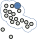
\includegraphics[width=4.2cm]{rolling-ball.pdf}
	\caption{The rolling ball method for cluster detection provides a way of
		identifying clusters, as inspired by molecular biology. A very simple
		implementation can be fast but is not particularly successful at
		finding clusters unless the data points are very dense and there is no
		noise.} \label{fig:rolling-ball}
\end{figure}

A simple approximation of this technique can be acheived by using the same
\texttt{open}-ing and \texttt{close}-ing processes as are described in
Section~\ref{sec:simple_grid_method}.

% Created:  Thu 10 Jul 2014 04:22 PM
% Modified: Thu 10 Jul 2014 04:22 PM
% @author Josh Wainwright
% File name : quadtree-traversal.tex

\section{Quadtree Traversal}
\label{sec:quadtree_traversal}

Whether the quadtree is stored in memory as a recursive quadtree data
structure, or as hash table, Section~\ref{sub:hash_table_implementation}, the
most important and computationally intensive step is extracting the clusters at
the correct depth and disregarding those data points that can be attributed to
noise.

The quadtree numbering system chosen lends itself very well to analysis based
on spatial location and the proximity of neighbours to a given cell being
examined. The neighbours of interest, named as \emph{rook's case} neighbours
% TODO Add abel and mark paper reference.
by~ref{}, are the four cells that lie to the north, east, sound and west of the
current

\begin{figure}[tbhp]
	\centering
	\includegraphics[width=0.88\linewidth]{propogation.pdf}
	% TODO caption
	\caption{Propagation}
	\label{fig:propogation}
\end{figure}

When discovering clusters via this propagation technique, care must be taken to
avoid a run-away situation where every node in the tree gets included. This
would happen when looking at the neighbours of a node and blindly including
them. Since every internal node has exactly four neighbours, the propagation
would terminate only when reaching the edge nodes.

Instead, the depth of the node must be considered. Again, the simplest method
is not sufficient. If the propagation is limited to a given node depth, even if
this is not the same as the deepest node, the size of any clusters that are
identified will be limited, as shown in Figure~\ref{fig:propogation-halting}.
Since the depth to consider is not able to change, when the neighbours of the
blue cell are checked, no correct neighbours are found and so the process
terminates. When able to view the larger structure of the cells, however, it is
clear that the structure continues beyond the gap.

\begin{figure}[tbhp]
	\centering
	\includegraphics[width=0.7\linewidth]{propogation-halting.pdf}
	\caption{propogation-Halting}
	\label{fig:propogation-halting}
\end{figure}

To avoid this, a certain amount of leniency must be given when deciding what
constitutes a neighbour. Given an appropriate value, this would allow both of
the larger white cells in Figure~\ref{fig:propogation-halting} to be included.

The \emph{depth range} shall define the levels that are to be considered when
choosing neighbours with respect to a target depth. Since clusters are being
considered areas of increased density of points, all cells with a depth greater
than the target depth shall be allowed, so the purple cells in
Figure~\ref{fig:propogation-halting} would be included when the target depth is
the same as the depth of the included red cells. A depth range of zero is
eqivalent to the situation above where only cells of a given depth are
considered. A depth range of 1 would mean that the white square in
Figure~\ref{fig:propogation-levels}\,b) would be included but not in~c),
whereas a depth range of three would include both.

\begin{figure}[tbhp]
	\centering
	\includegraphics[width=0.88\linewidth]{propogation-levels.pdf}
	\caption{propogation-Levels}
	\label{fig:propogation-levels}
\end{figure}


% Created:  Thu 10 Jul 2014 04:22 PM
% Modified: Thu 10 Jul 2014 04:22 PM
% @author Josh Wainwright
% File name : quadtree-traversal.tex

\section{Quadtree Traversal}
\label{sec:quadtree_traversal}

Whether the quadtree is stored in memory as a recursive quadtree data
structure, or as hash table, Section~\ref{sub:hash_table_implementation}, the
most important and computationally intensive step is extracting the clusters at
the correct depth and disregarding those data points that can be attributed to
noise.

The quadtree numbering system chosen lends itself very well to analysis based
on spatial location and the proximity of neighbours to a given cell being
examined. The neighbours of interest, named as \emph{rook's case} neighbours
% TODO Add abel and mark paper reference.
by~ref{}, are the four cells that lie to the north, east, sound and west of the
current

\begin{figure}[tbhp]
	\centering
	\includegraphics[width=0.88\linewidth]{propogation.pdf}
	% TODO caption
	\caption{Propagation}
	\label{fig:propogation}
\end{figure}

When discovering clusters via this propagation technique, care must be taken to
avoid a run-away situation where every node in the tree gets included. This
would happen when looking at the neighbours of a node and blindly including
them. Since every internal node has exactly four neighbours, the propagation
would terminate only when reaching the edge nodes.

Instead, the depth of the node must be considered. Again, the simplest method
is not sufficient. If the propagation is limited to a given node depth, even if
this is not the same as the deepest node, the size of any clusters that are
identified will be limited, as shown in Figure~\ref{fig:propogation-halting}.
Since the depth to consider is not able to change, when the neighbours of the
blue cell are checked, no correct neighbours are found and so the process
terminates. When able to view the larger structure of the cells, however, it is
clear that the structure continues beyond the gap.

\begin{figure}[tbhp]
	\centering
	\includegraphics[width=0.7\linewidth]{propogation-halting.pdf}
	\caption{propogation-Halting}
	\label{fig:propogation-halting}
\end{figure}

To avoid this, a certain amount of leniency must be given when deciding what
constitutes a neighbour. Given an appropriate value, this would allow both of
the larger white cells in Figure~\ref{fig:propogation-halting} to be included.

The \emph{depth range} shall define the levels that are to be considered when
choosing neighbours with respect to a target depth. Since clusters are being
considered areas of increased density of points, all cells with a depth greater
than the target depth shall be allowed, so the purple cells in
Figure~\ref{fig:propogation-halting} would be included when the target depth is
the same as the depth of the included red cells. A depth range of zero is
eqivalent to the situation above where only cells of a given depth are
considered. A depth range of 1 would mean that the white square in
Figure~\ref{fig:propogation-levels}\,b) would be included but not in~c),
whereas a depth range of three would include both.

\begin{figure}[tbhp]
	\centering
	\includegraphics[width=0.88\linewidth]{propogation-levels.pdf}
	\caption{propogation-Levels}
	\label{fig:propogation-levels}
\end{figure}

% Created:  TIMESTAMP
% Modified: TIMESTAMP

\section{ImageJ Plugin}
\label{sec:imagej_plugin}

\subsection{ImageJ}
\label{sub:imagej}

Imagej is an public domain, Java based image manipulation program written and
maintained by developers at the National Institute of Health. It is widly used
in medical and biological research and has an open API to allow extension via
macros, plugins and scripts.

Since they offer significantly betting integration, meaning speed and
efficiency improvements, a plugin is chosen to inegrate this project into
ImageJ over macros, which suffer performace loss when more than a few steps are
involved, and scripts which do not offer such tight integration with the rest of
the program.

The plugin shall allow a user to load a data set, as gathered from STORM, PALM
or similar imaging techniques discussed in
Section~\ref{sec:sub_diffraction_limit_imaging}, analyse the data for clusters
and receive detailed information regarding the clusters that were found.

% Created:  Fri 04 Jul 2014 04:47 PM
% Modified: Tue 29 Jul 2014 12:23 PM
% @author Josh Wainwright
% File name : imagej_plugin.tex

\section{ImageJ Plugin}
\label{sec:imagej_plugin}

% TODO section about the aims of the plugin etc.
\cite{imagejapi}

\subsection{Displaying the QuadTree}
\label{sub:displaying_the_quadtree}

The first version of the plugin simply allowed the user to visualise the data,
once it had been processed and entered into a quadtree. Though this provided
little benefit to the researcher producing data, it can be a useful tool to get
an insight into the process that a program is using to analyse one's data so
that the results can be better interpreted. For this reason, this version
served as a foundation for later versions of the plugin so that, when loading
data, a user gets the opportunity to view the data before proceeding with the
analysis.

Again, earlier versions of the program displayed this data using the built-in
GUI classes in the AWT\cite{zukowski1997java} and Swing\cite{loy2002java}
libraries included in the standard Java distribution. This effectively
prohibited any further actions being performed on the image once it had been
generated since what was displayed was only modifiable by the JVM via compiled
code. It was also very memory intensive since, in many cases, many thousands of
separate objects (data points represented by zero length lines, quadtree cells
by boxes, etc.) and so was slow to draw initially and redraw with any
subsequent move or resize of the window.

The code used to generate this view of the data was modified to make use of the
easy image generation functions present in ImageJ. Now, instead of many
different objects being manipulated for each view of the data, a single array
with a value for each pixel is needed. For the cases where the user wishes to
view the clusters that have been found, but not have them affect the image, the
image is created with a number of different \emph{slices} in the image
\emph{stack}, Figure~\ref{fig:imagej-stack}. Slices are ImageJ's representation
of images with two or more layers, or alternative views, each of which resides
in a stack of slices. Each slice in a stack must have the same dimensions.

\begin{figure}[tbhp]
	\centering
	\includegraphics[width=0.8\linewidth]{imagej-stack.pdf}
	% TODO caption
	\caption{imagej-Stack}
	\label{fig:imagej-stack}
\end{figure}

\subsection{Column Picker}
\label{sub:column_picker}

% TODO writing about column picker

\subsection{Results Table}
\label{sub:results_table}

In addition to the image of the data with the clusters, the plugin also
calculates a number of statistics for each of the clusters that are found.
These include the number of points that are included in the cluster, the area
of the cluster, and it's perimeter. The area and perimeter values are given as
a fraction where the whole image represents 1. Thus, to find the actual area
for the real life object, the area of the cluster should be multiplied by the
area of the image, and for the perimeter, the length of one side of the image
should be multiplied by the perimeter.

To calculate each of these values, each node that exists in a cluster is
examined and its contribution to the overall value added.

\subsubsection{Cluster Area}
\label{ssub:Cluster Area}

To calculate the area of the clusters, each node in each cluster is examined.
Since the size of the node must be known, it is calculated from the quadtree
code for that node. The formula is shown in Equation~\ref{eq:node-area},
\begin{align}
	a &= \frac{1}{4^{d}} \\
	a_i &= 4^{-l_i/2}, \label{eq:node-area}
\end{align}
where $a_i$ is the area of the node $i$, $d$ is the depth in the quadtree and
$l_i$ is the length of the quadtree code of that node. For every node in the
cluster, where there are $n$ nodes, this value is summed to give the total
cluster area, $A$:
\begin{align}
	A &= \sum_{i=0}^{n} a_i.
\end{align}

\subsubsection{Cluster Perimeter}
\label{ssub:Cluster Perimeter}

Similarly to the cluster area, the perimeter is given as a fractional value of
the length of one side of the whole image, as calculated for each node from the
quadtree code, as shown in Equation~\ref{eq:node-perimeter},
\begin{align}
	p &= \frac{1}{2^{d}} \\
	p_i &= 2^{-l_i/2}, \label{eq:node-perimeter}
\end{align}
where the symbols have the same meaning as above.

However, this simply gives the length of one side of the node for any node. In
order to calculate the perimeter of the cluster, it is not enough to simply
sum these values, as for the cluster area, since not all nodes contribute to
the perimeter. Instead, for each node, it must be decided whether it
contributes to the perimeter and how much (1, 2, 3 or 4 sides), and then
increase the total perimeter by this many times the length of one side. The
total perimeter, $P$, then is given by Equation~\ref{eq:total-perimeter},
\begin{align}
	P &= \sum_{i=0}^{n} s * p_i, \label{eq:total-perimeter}
\end{align}
where $s \in \{0..4\}$. This is demonstrated in
Figure~\ref{fig:perimeter-edges} where the perimeter is simple to calculate in
case a) as the nodes are all the same, but the size of each node must be taken
into account in case b).

\begin{figure}[tbhp]
	\centering
	\includegraphics[width=0.8\linewidth]{perimeter-edges.pdf}
	\caption{When calculating the perimeter of a cluster using the nodes that
		contribute, the size of each node must be taken into account. In case
		a), the process is simple since all nodes are the same size and a
		fractional value of 3.5 is calculated. For case b), the steps are 25
		lengths of size $\rfrac{1}{8}$ and 6 lengths of size $\rfrac{1}{16}$
		which gives the same result, 3.5.} \label{fig:perimeter-edges}
\end{figure}

Within the cluster, \emph{holes} occur where a node, or number of nodes, is
surrounded on all sides by the same cluster. An example can be seen in
Figure~\ref{fig:kernel-options}. Unfortunately, these are included in the
calculation of the perimeter and so, where holes exist in a cluster, the actual
perimeter is slightly smaller than that calculated.


\clearpage
% Created:  Sun 15 Jun 2014 04:27 pm
% Author:   Josh Wainwright
% Filename: appendix.tex

\appendix

\part{Appendix}
\label{prt:appendix}

% Created:  Mon 25 Aug 2014 02:12 pm
% Author:   Josh Wainwright
% Filename: running-plugin.tex

\section{Compiling and Running the Plugin}
\label{sec:running_the_plugin}

The steps required to compile the plugin are given below. These steps require
Apache Ant to be installed with a relatively recent version of the JavaVM\@.
\begin{enumerate}
	\item Edit the \texttt{build.xml} file to change the third line with the
		\texttt{imagej-plugin-location} variable to point to the ``jars''
		folder within the plugin section of the ImageJ executable folder.
	\item Run the command \texttt{ant compile} from the same folder as the
		\texttt{build.xml} file to compile the Java source and generate the
		Java jar file ready for installation.
	\item If there were no errors, run the command \texttt{ant imagej} to copy
		the generated jar file to the relavent folder to be run by ImageJ.
	\item The command \texttt{ant imagej} can be run to both compile and copy
		the file.
\end{enumerate}

To run the plugin from ImageJ, follow the steps below.
\begin{enumerate}
	\item If ImageJ is already running when the plugin was installed, refresh
		the menus so that the latest version of the plugin by clicking
		\texttt{Help >> Refresh Menus}.
	\item Run the plugin by clicking \texttt{Plugins >> jars >> Cluster
		Analysis}.
\end{enumerate}

\newpage
% Created:  Mon 23 Jun 2014 04:06 PM
% Modified: Sun 10 Aug 2014 11:12 am
% @author Josh Wainwright
% File name : file-columns.tex

\section{Data File Structure}
\label{app:data_file_structure}

The data files that are produced from the initial analysis of the images have a
standard format.

\begin{enumerate}
	\item Tab separated fields.
	\item Single header line with names of fields.
	\item One or more item of data, separated by newlines.
\end{enumerate}

The columns that represent fields in the file are as follows.

\begin{center}
	\begin{tabu}{p{1.1cm} X c}
		\toprule
		Header & Meaning & Used? \\
		\midrule
		\texttt{Channel Name} & Wavelength channel that was used to capture data.
			First value, $I$, is the incident wavelength of the light used to
			excite the dye and the second, $E$, is the wavelength emitted that
			was imaged. & no \\
		\texttt{X} & x-coordinate of the point & no \\
		\texttt{Y} & y-coordinate of the point & no \\
		\texttt{Xc} & centered, normalised x-coordinate of point & yes \\
		\texttt{Yc} & centered, normalised y-coordinate of point & yes \\
		\texttt{Height} & the height of the fitted gaussian peak used to
			extract the point from the original image & not yet \\
		\texttt{Area} & area of the point & not yet \\
		\texttt{Width} & full width half maximum of the point & not yet \\
		\texttt{Phi}          &  & no \\
		\texttt{Ax}           &  & no \\
		\texttt{BG}           &  & no \\
		\texttt{I}            &  & no \\
		\texttt{Frame}        &  & no \\
		\texttt{Length}       &  & no \\
		\texttt{Valid}        &  & no \\
		\texttt{Z}            &  & no \\
		\texttt{Zc}           &  & no \\
		\texttt{Photons}      &  & no \\
		\texttt{Lateral Localisation Accuracy}     &  & no \\
		\texttt{Xw}           &  & no \\
		\texttt{Yw}           &  & no \\
		\texttt{Xwc}          &  & no \\
		\texttt{Ywc}          &  & no \\
		\bottomrule
	\end{tabu}
\end{center}

\newpage
% Created:  Mon 25 Aug 2014 10:11 am
% Author:   Josh Wainwright
% Filename: benchmark-hardware.tex

\section{Benchmarking Hardware}
\label{sec:benchmarking_hardware}

The benchmarking of algorithms to get time to run information was performed on
hardware with the following specifications, as recorded by the \texttt{lscpu}
utility from the util-linux package\cite{lscpu}.

% TODO system information of benchmark machine
%
\begin{tabular}{l l}
	Architecture:          & x86\_64 \\
	CPU op-mode  (s):      & 32-bit, 64-bit \\
	Byte Order:            & Little Endian \\
	CPU (s):               & 4 \\
	On-line CPU (s) list:  & 0--3 \\
	Thread (s) per core:   & 1 \\
	Core (s) per socket:   & 4 \\
	Socket (s):            & 1 \\
	NUMA node (s):         & 1 \\
	Vendor ID\@:           & GenuineIntel \\
	CPU family:            & 6 \\
	Model:                 & 60 \\
	Stepping:              & 3 \\
	CPU MHz:               & 800.000 \\
	BogoMIPS\@:            & 6385.81 \\
	Virtualization:        & VT-x \\
	L1d cache:             & 32K \\
	L1i cache:             & 32K \\
	L2 cache:              & 256K \\
	L3 cache:              & 6144K \\
	NUMA node0 CPU (s):    & 0--3 \\
\end{tabular}

\newpage
% Created:  Sat 02 Aug 2014 06:48 pm
% Modified: Mon 04 Aug 2014 04:09 PM
% @author Josh Wainwright
% File name : roundness.tex

\section{Roundness Derivation}
\label{app:roundness_derivation}

Derivation of the equation for roundness, $R$, of a cluster given the area,
$A$, and perimeter, $p$, of the cluster.

A circle is defined to have a roundness of 1.

\begin{align}
	R_\textrm{circle} = 1 \\
\intertext{The value must be unitless, so divide area by perimeter squared,}
	A &= \pi r^2 \\
	p &= 2\pi r \\
	\frac{A}{p} &= \frac{\pi r^2}{4\pi^2 r^2} \\
\intertext{Remove constants to give formula,}
	R &= 4\pi\frac{\pi r^2}{4\pi^2 r^2} \\
		&= 4\pi \frac{A}{p}
\end{align}

Test for regular shapes.

\paragraph{Circle}
\label{par:circle}

\begin{align}
	A &= \pi r^2 \\
	p &= 2\pi r \\
	R &= 4\pi \times \frac{\pi r^2}{(2\pi r)^2} = 1
\end{align}

\paragraph{Square}
\label{par:square}

\begin{align}
	A &= h^2 \\
	p &= 4h \\
	R &= 4\pi \times \frac{h^2}{(4h)^2} = \frac{\pi}{4} \approx 0.785
\end{align}

\paragraph{Equalateral Triangle}
\label{par:equalateral_triangle}

\begin{align}
	A &= \frac{\sqrt{3}}{4}a^2 \\
	p &= 3h \\
	R &= 4\pi \times \frac{\frac{\sqrt{3}}{4}a^2}{(3a)^2} = \frac{\sqrt{3}\pi}{9} \approx 0.605
\end{align}

\paragraph{Elipse ($\textrm{Eccentricity} = 0.5$)}
\label{par:elipse}

For ellipse, $\epsilon = 0.5$, let minor axis, $a = 1$ and major axis, $b = 2$.
\begin{align}
	A &= 6.28 \\
	p &= 9.69 \\
	R &= \frac{6.28}{9.69} \approx 0.648
\end{align}

\newpage
% Created:  Wed 23 Jul 2014 11:30 AM
% Modified: Wed 23 Jul 2014 11:30 AM
% @author Josh Wainwright
% File name : class-diagram.tex

\section{Class Diagram}
\label{sec:class_diagram}

Figure~\ref{fig:class-diagram} is a class diagram showing the structure of the
ImageJ plugin that was created for this project.

\begin{figure*}[tbhp]
	\centering
	\includegraphics[angle=90,height=\textheight]{plugin_class_diagram.pdf}
	% TODO caption
	\caption{}
	\label{fig:class-diagram}
\end{figure*}

\newpage
% Created:  Sat 02 Aug 2014 06:48 pm
% Modified: Mon 04 Aug 2014 04:36 PM
% @author Josh Wainwright
% File name : flow-diagram.tex

\section{Flow Diagram}
\label{sec:flow_diagram}

Figure~\ref{fig:flow-diagram} is a flow diagram showing the flow of events from
initialisation of the plugin from ImageJ through to drawing the clusters found
to an image of the data set on screen.

% 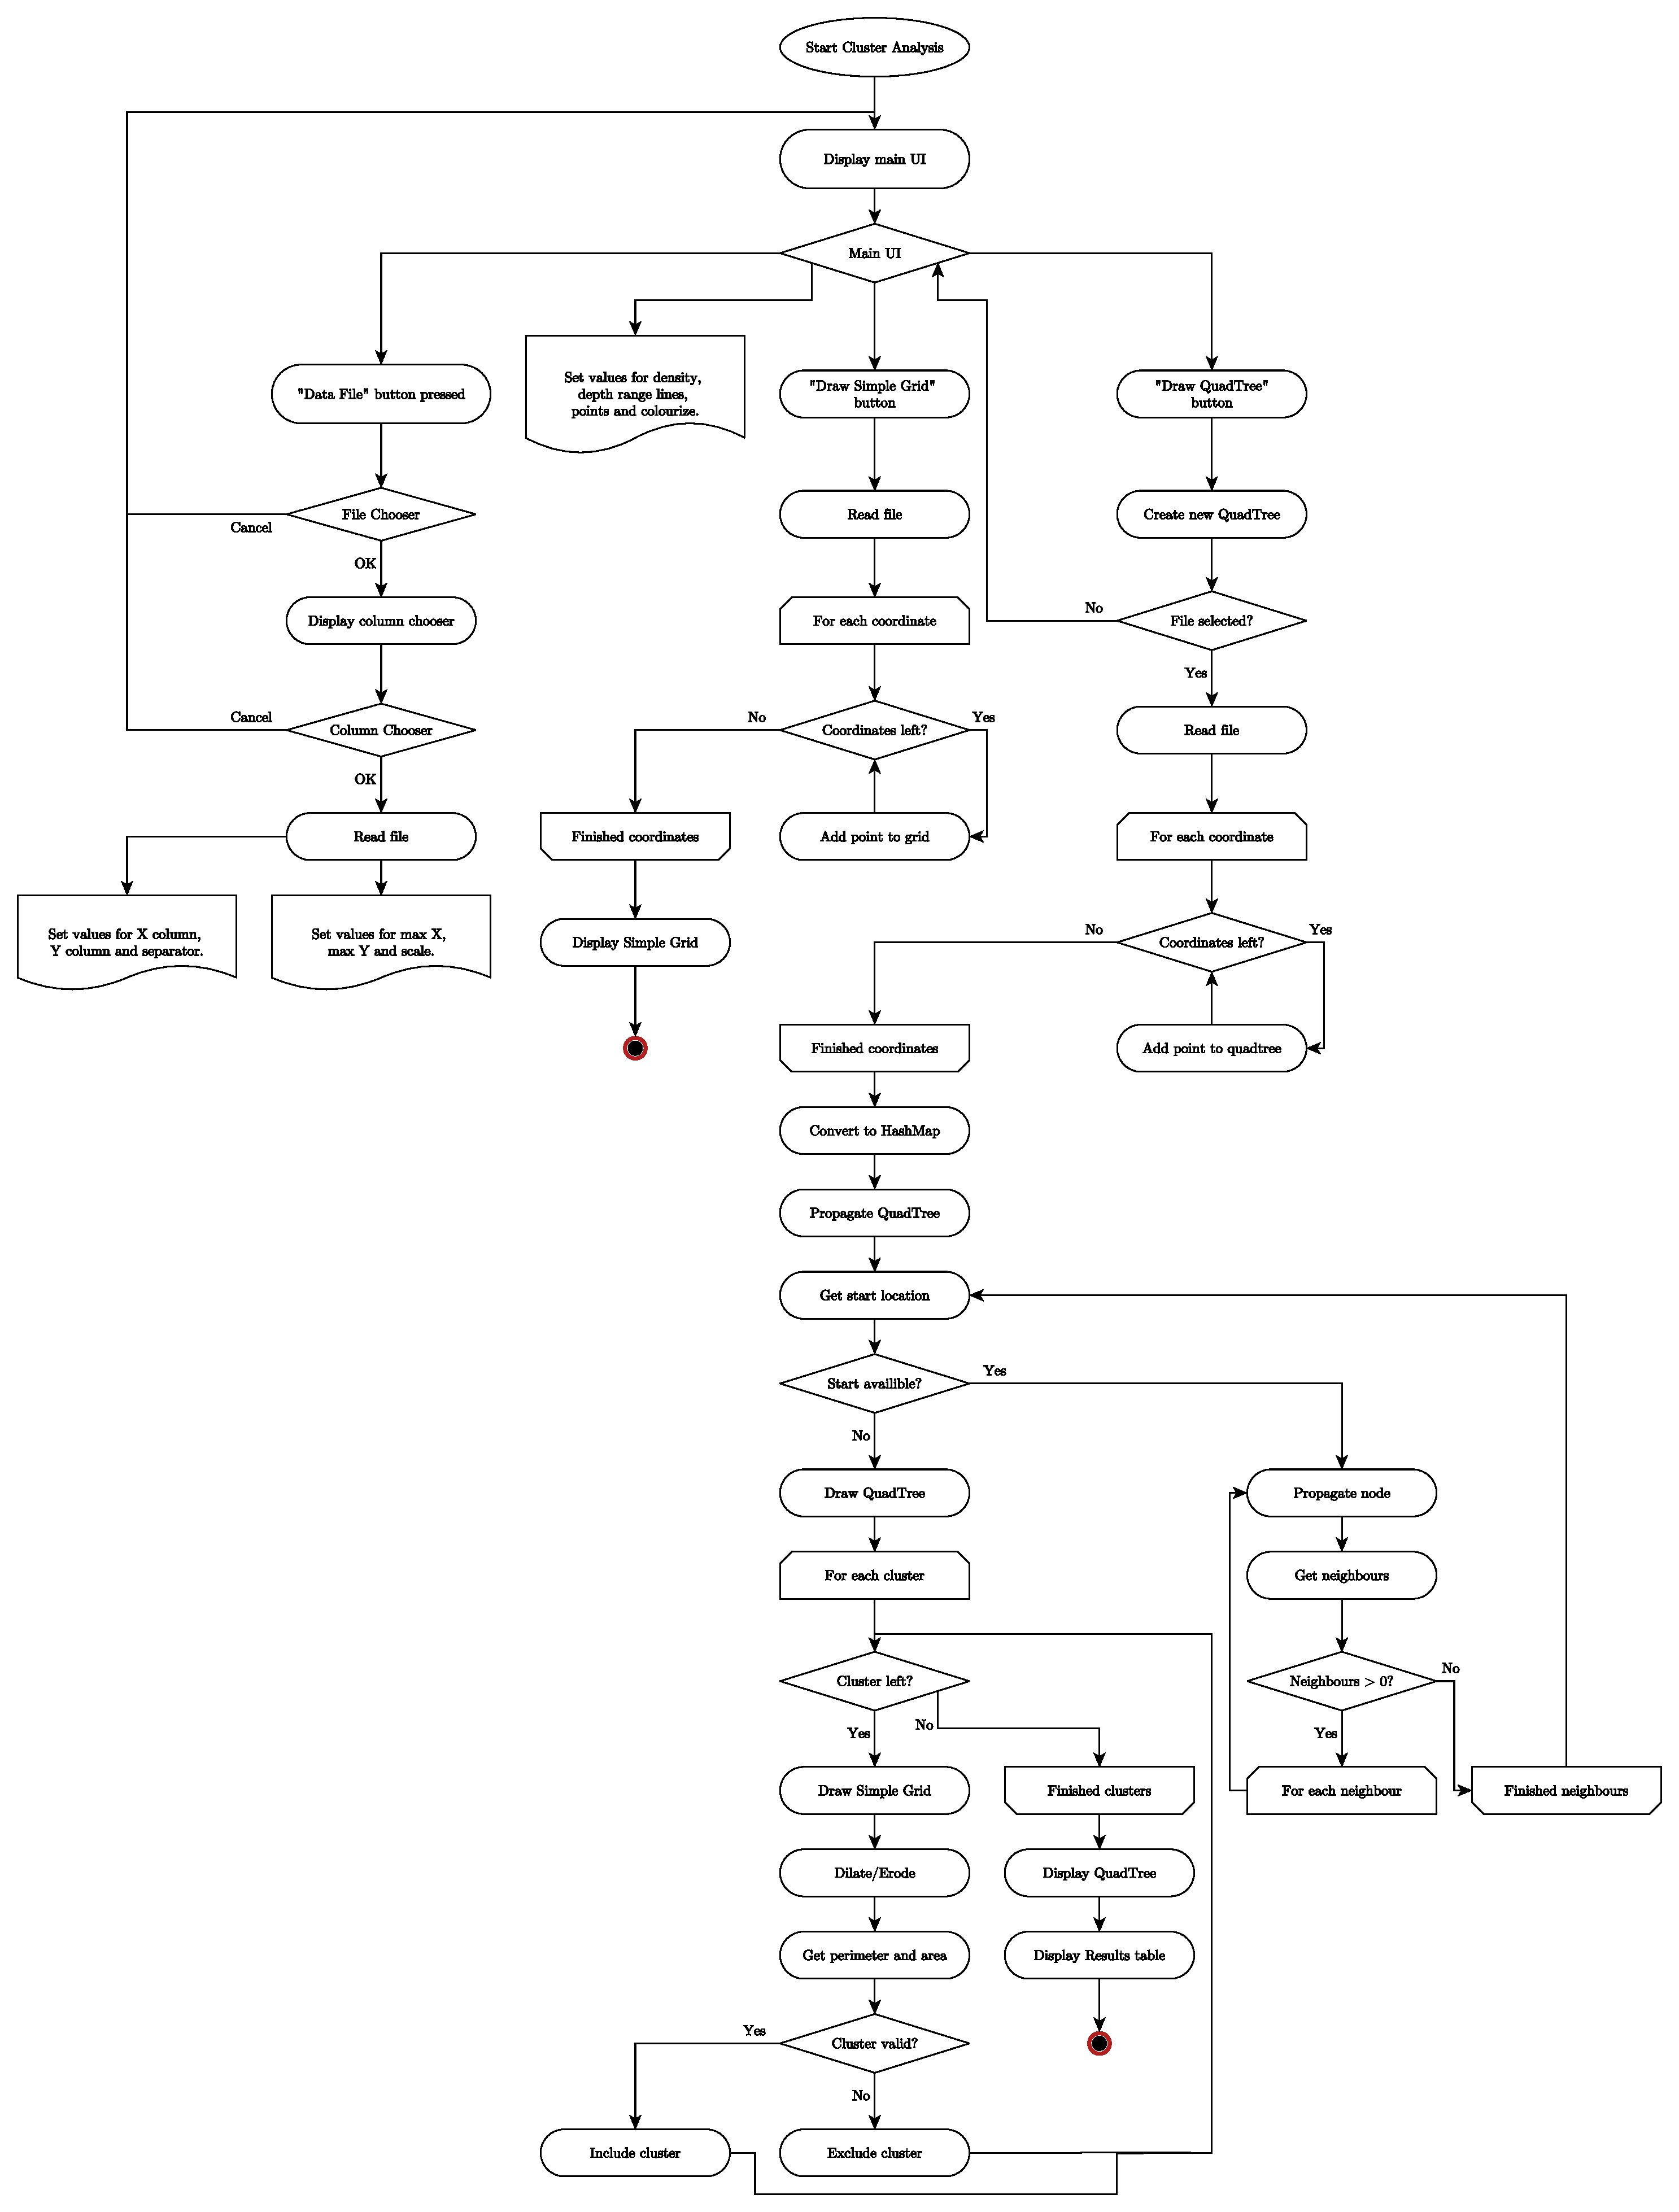
\includegraphics[width=\textwidth]{flow-chart.pdf}
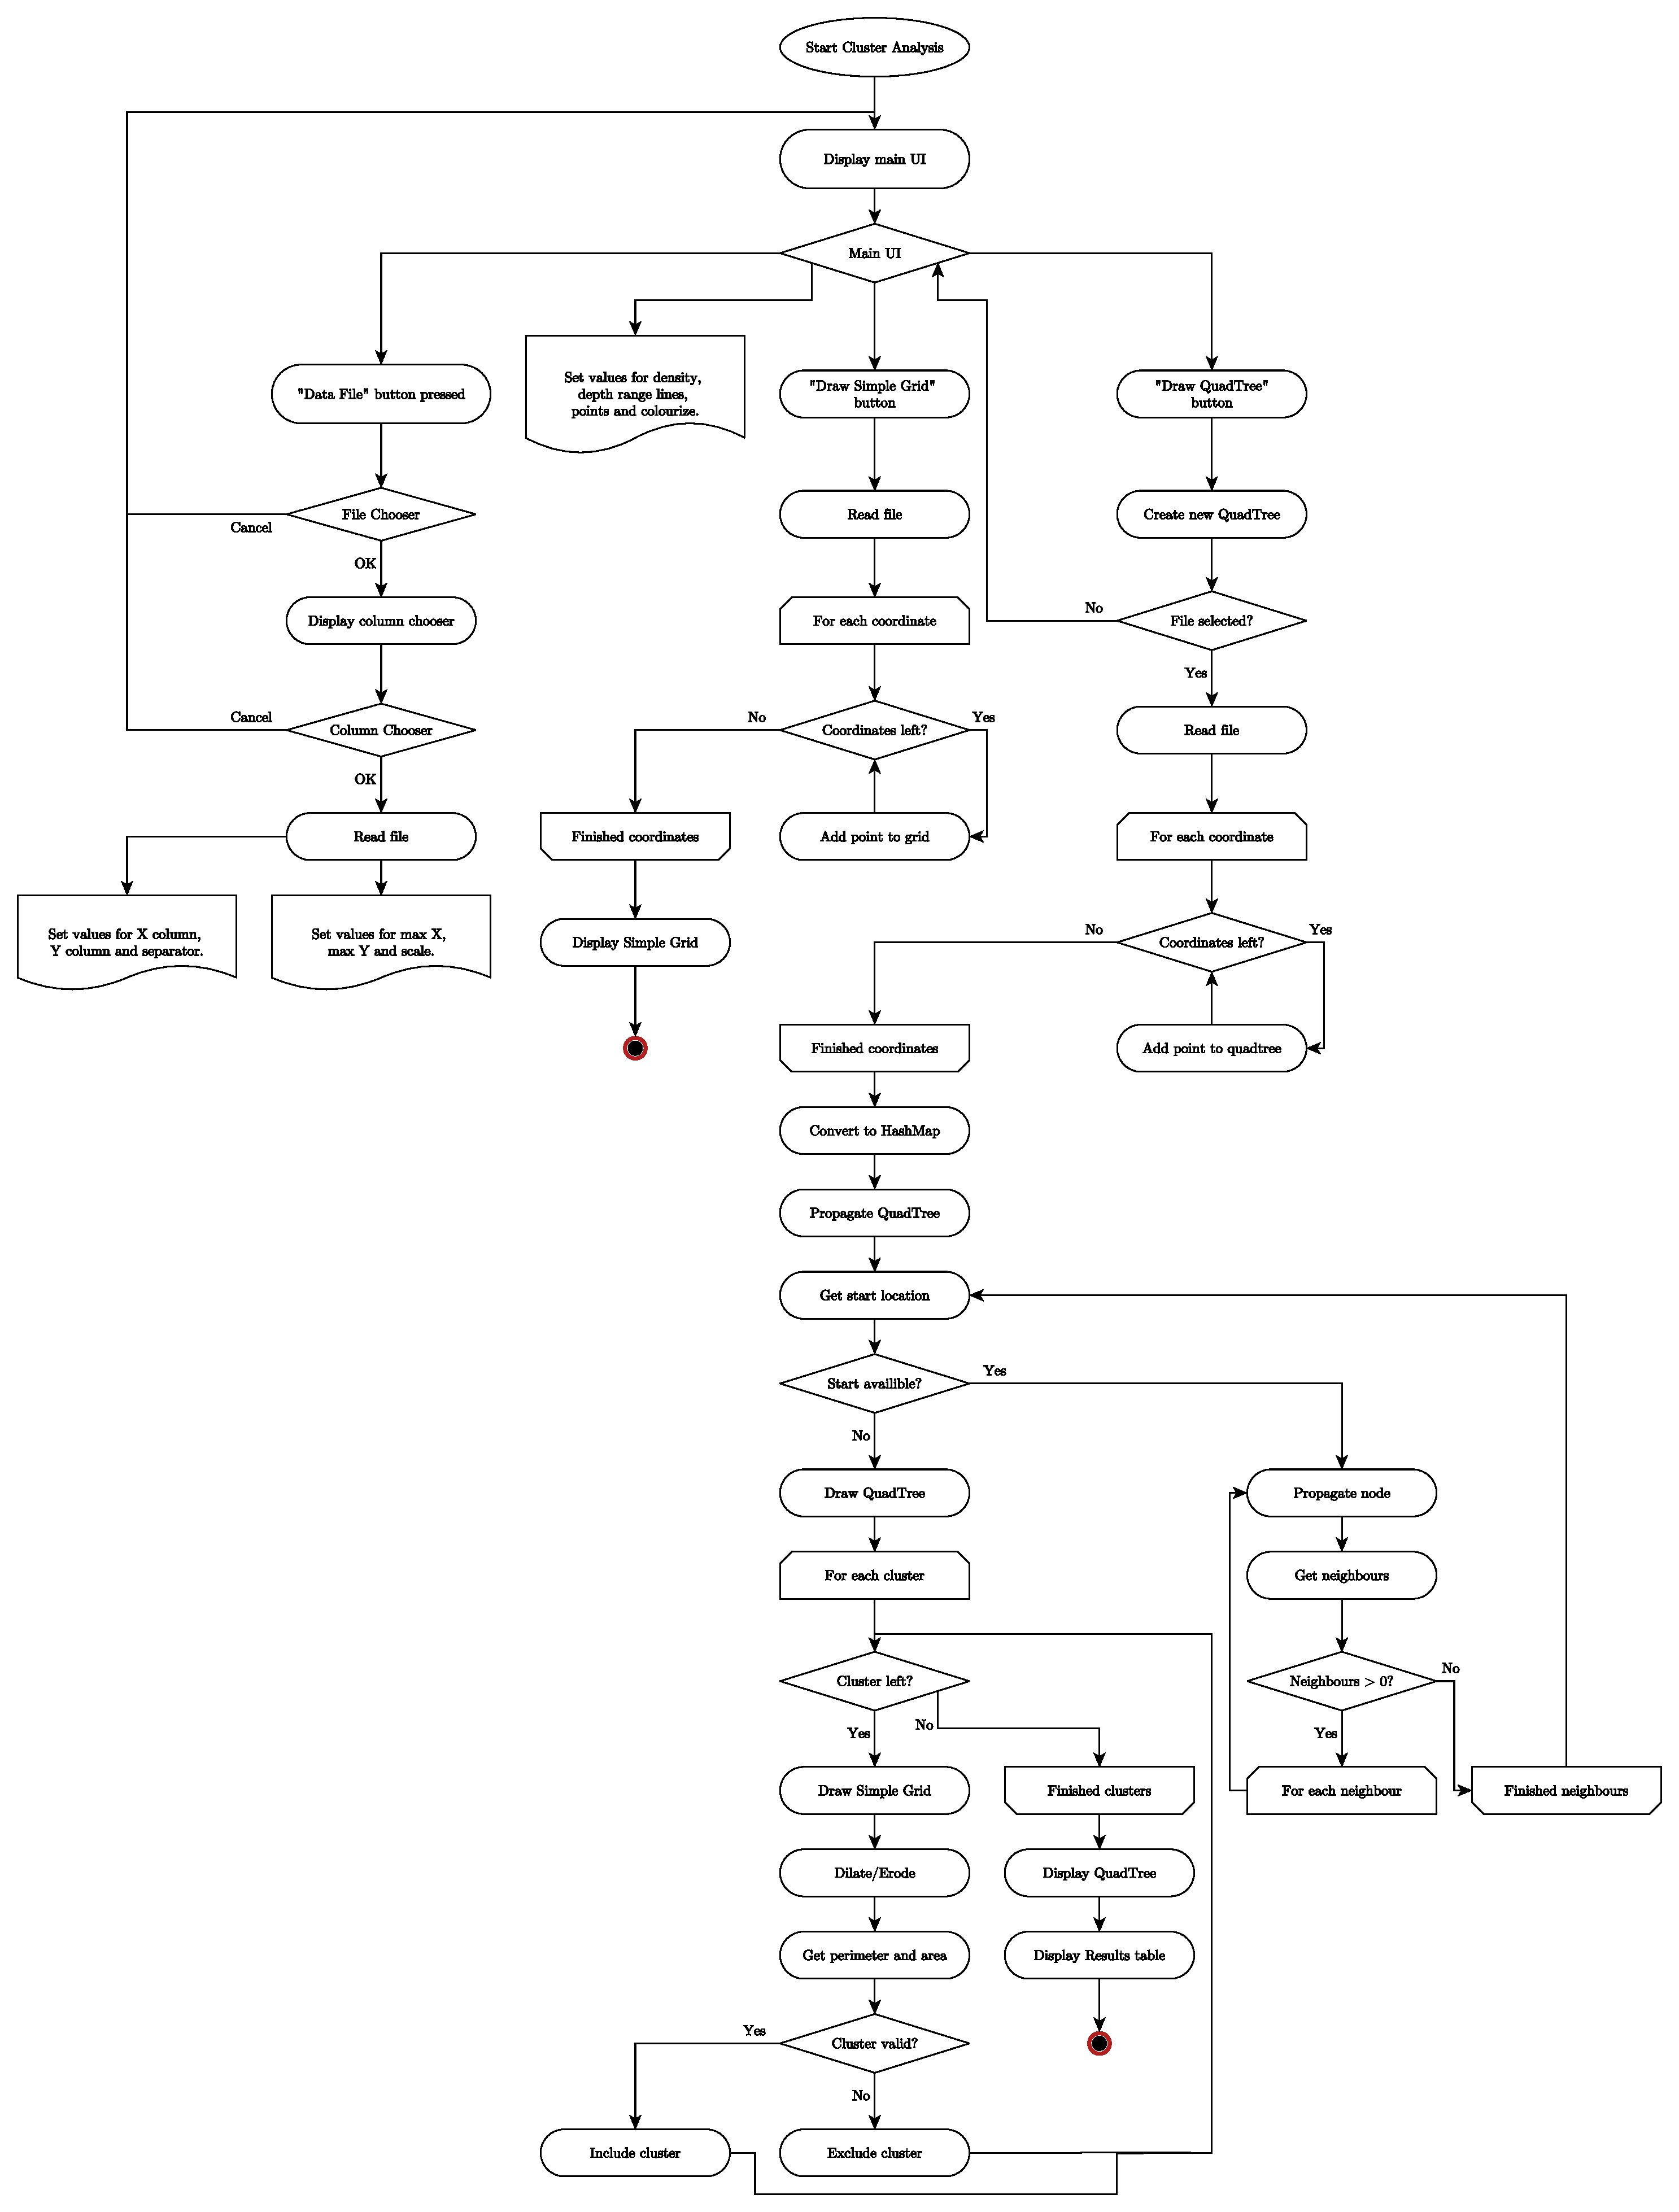
\includegraphics[height=0.9\textheight]{flow-chart.pdf}\label{fig:flow-diagram}

\newpage
% Created:  Mon 04 Aug 2014 04:49 PM
% @author Josh Wainwright
% File name : add-point-flow.tex

\section{Add-point Flow Diagram}
\label{sec:add_point_flow_diagram}

Figure~\ref{fig:add-point-flow-diagram} is a flow diagram showing the flow of
events from initialisation of the plugin from ImageJ through to drawing the
clusters found to an image of the data set on screen.

\begin{figure*}[tbhp]
	\centering
	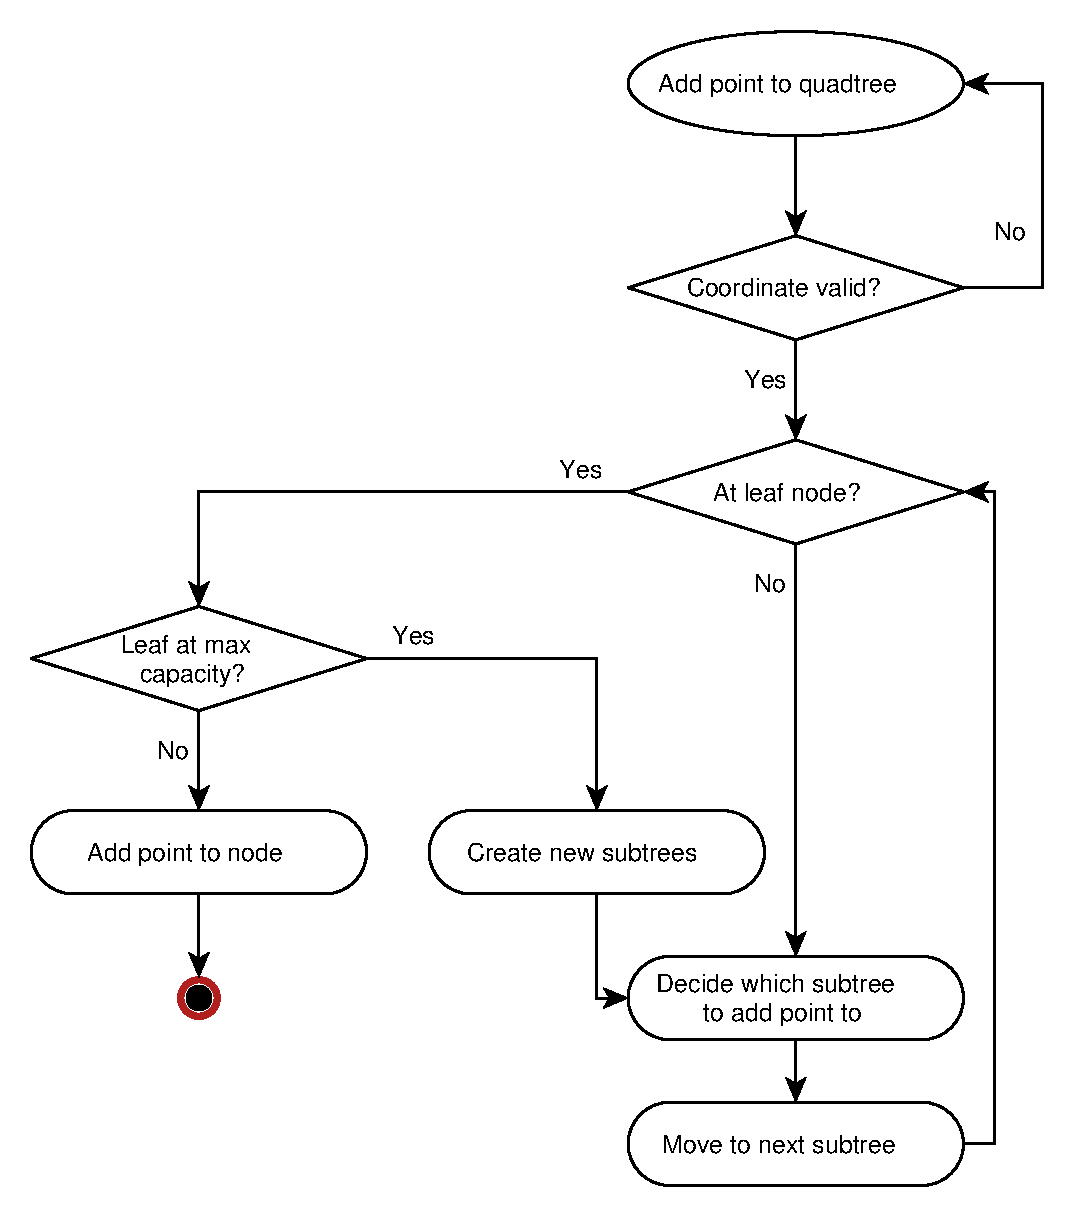
\includegraphics[width=0.5\textwidth]{add-point-flow-chart.pdf}
	% 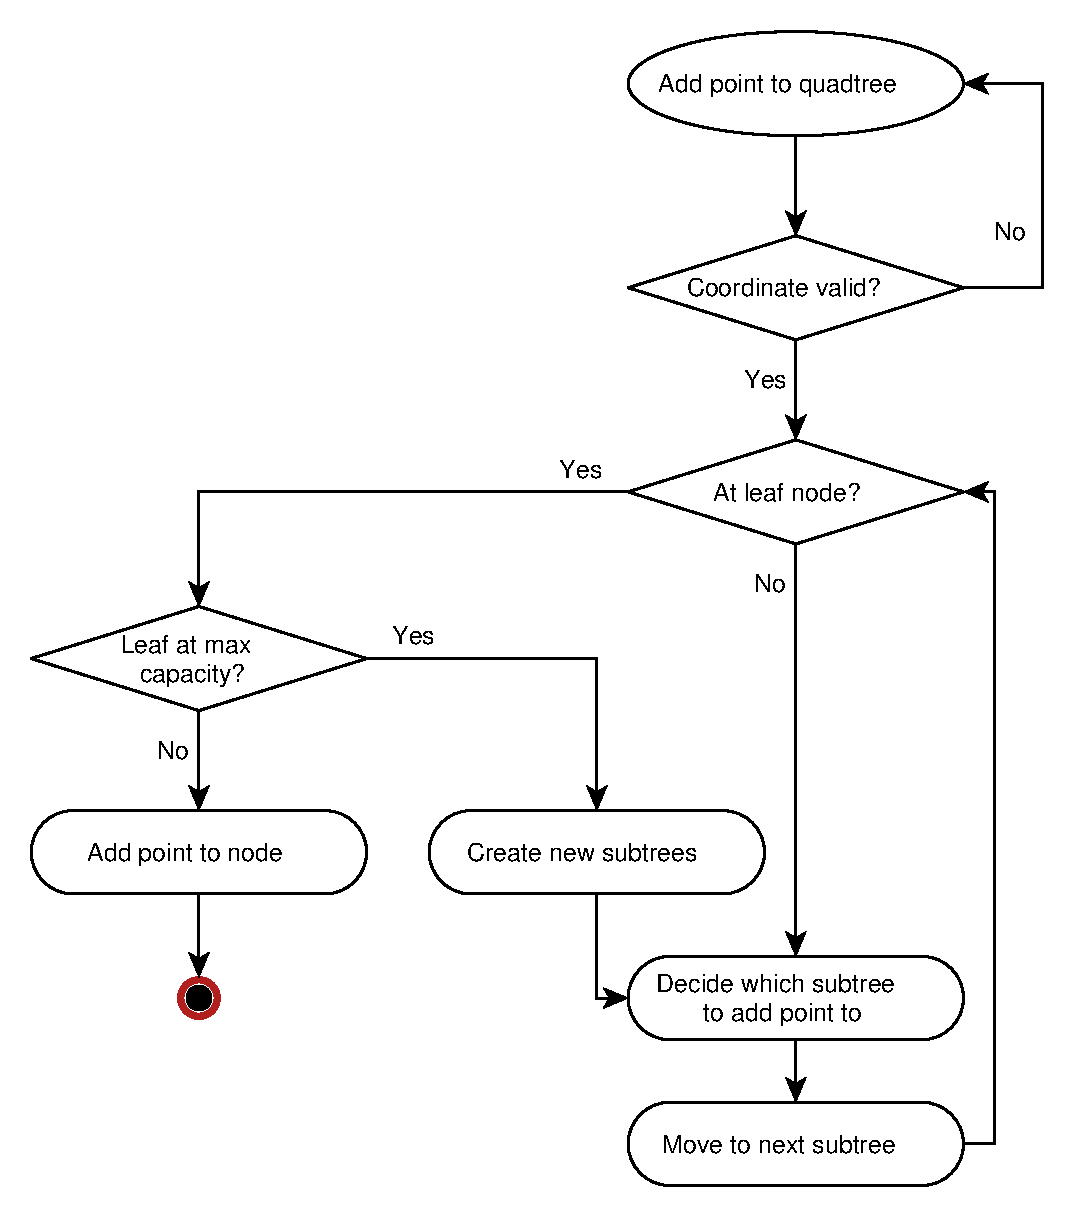
\includegraphics[height=\textheight]{add-point-flow-chart.pdf}

	\caption{Class diagram for the Cluster Analysis ImageJ plugin written for
	this project.}\label{fig:add-point-flow-diagram}
\end{figure*}



% \clearpage
\newgeometry{onecolumn,top=2in,left=1.5in,right=1.5in}
\thispagestyle{empty}
\nocite{*}
\bibliographystyle{apalike}
\bibliography{references}
\restoregeometry

\end{document}
